\documentclass[english]{article}
\usepackage[latin9]{inputenc}
\usepackage{amsmath}
\usepackage{amssymb}
\usepackage{xargs}[2008/03/08]
\usepackage{babel}
\usepackage{tikz}
\begin{document}
% TODO: change def to newcommand

% sectioning and structure
% \theoremstyle{italic}
\newtheorem{theorem}{Theorem}[section]
\newtheorem{assumption}[theorem]{Assumption}
\newtheorem{lemma}[theorem]{Lemma}
\newtheorem{claim}[theorem]{Claim}
\newtheorem{problem}[theorem]{Problem}
%\newtheorem{algorithm}[theorem]{Algorithm}
\newtheorem{proposition}[theorem]{Proposition}
\newtheorem{corollary}[theorem]{Corollary}
\newtheorem{construction}[theorem]{Construction}
\newtheorem{definition}[theorem]{Definition}
\newtheorem{example}[theorem]{Example}
\newtheorem{xca}[theorem]{Exercise}
\newtheorem{comments}[theorem]{Comments}
\newtheorem{remark}[theorem]{Remark}
\newtheorem{thm}{\protect\theoremname}
%\theoremstyle{plain}
\newtheorem{lem}[thm]{\protect\lemmaname}

\newcommand{\zerob}{\mathbf{0}}
\newcommand{\oneb}{\mathbf{1}}%

\newcommand{\snr}{\text{SNR}}
\global\long\def\norma#1{\left\Vert #1\right\Vert }%

\newcommand{\Ab}{\mathbf{A}}%
\newcommand{\ab}{\mathbf{a}}%

\newcommand{\Bb}{\mathbf{B}}%
\newcommand{\bb}{\mathbf{b}}%

\newcommand{\Cb}{\mathbf{C}}%
\newcommand{\cb}{\mathbf{c}}%

\newcommand{\Db}{\mathbf{D}}%
\newcommand{\db}{\mathbf{d}}%

\newcommand{\Eb}{\mathbf{E}}%
\newcommand{\eb}{\mathbf{e}}%

\newcommand{\Fb}{\mathbf{F}}%
\newcommand{\fb}{\mathbf{f}}%

\newcommand{\Gb}{\mathbf{G}}%
\newcommand{\gb}{\mathbf{g}}%

\newcommand{\Hb}{\mathbf{H}}%
\newcommand{\hb}{\mathbf{h}}%

\newcommand{\Ib}{\mathbf{I}}%
\newcommand{\ib}{\mathbf{i}}%

\newcommand{\Jb}{\mathbf{J}}%
\newcommand{\jb}{\mathbf{j}}%

\newcommand{\Kb}{\mathbf{K}}%
\newcommand{\kb}{\mathbf{k}}%

\newcommand{\Lb}{\mathbf{L}}%
\newcommand{\lb}{\mathbf{l}}%

\newcommand{\Mb}{\mathbf{M}}%
\newcommand{\mb}{\mathbf{m}}%

\newcommand{\Nb}{\mathbf{N}}%
\newcommand{\nb}{\mathbf{n}}%

\newcommand{\Ob}{\mathbf{O}}%
\newcommand{\ob}{\mathbf{o}}%

\newcommand{\Pb}{\mathbf{P}}%
\newcommand{\pb}{\mathbf{p}}%

\newcommand{\Qb}{\mathbf{Q}}%
\newcommand{\qb}{\mathbf{q}}%

\newcommand{\Rb}{\mathbf{R}}%
\newcommand{\rb}{\mathbf{r}}%

\newcommand{\Sb}{\mathbf{S}}%
\renewcommand{\sb}{\mathbf{s}}%

\newcommand{\Tb}{\mathbf{T}}%
\newcommand{\tb}{\mathbf{t}}%

\newcommand{\Ub}{\mathbf{U}}%
\newcommand{\ub}{\mathbf{u}}%

\newcommand{\Vb}{\mathbf{V}}%
\newcommand{\vb}{\mathbf{v}}%

\newcommand{\Wb}{\mathbf{W}}%
\newcommand{\wb}{\mathbf{w}}%

\newcommand{\Xb}{\mathbf{X}}%
\newcommand{\xb}{\mathbf{x}}%

\newcommand{\Yb}{\mathbf{Y}}%
\newcommand{\yb}{\mathbf{y}}%

\newcommand{\Zb}{\mathbf{Z}}%
\newcommand{\zb}{\mathbf{z}}%

\newcommand{\RF}{\mathbb{R}}% rationals

\newcommand{\CF}{\mathbb{C}}% complex

\newcommand{\IF}{\mathbb{I}}% imaginary

\newcommand{\NF}{\mathbb{N}}% natural

\newcommand{\define}{\triangleq}%
\newcommand{\const}{\text{const}}%
\newcommand{\argThis}[3]
{
	\underset{#2}{#1}
	\left \lbrace #3 \right \rbrace
}
\newcommand{\argmax}[2]{\argThis{\text{argmax}}{#1}{#2}}
\newcommand{\argmin}[2]{\argThis{\text{argmin}}{#1}{#2}}
\newcommand{\defineInline}[2]{\underset{#2}{\underbrace{#1}}}
% Shortcuts and operators

\renewcommand{\=}[1]{\underset{#1}{=}}%

\newcommand{\intX}{\intop_{\Omega}}%
\newcommand{\inttheta}{\intop_{\Theta}}%
\newcommand{\intone}{\intop_{-1}^{1}}%
\newcommand{\intinf}{\intop_{-\infty}^{\infty}}%

% Statistics
\newcommand{\tetahat}{\hat{\boldsymbol{\theta}}}%
\newcommand{\cnormaldistribution}[2]{\mathcal{N}^{c}\left(#1,#2\right)}%
\newcommand{\normaldistribution}[2]{\mathcal{N}\left(#1,#2\right)}%
\renewcommand{\tt}{\boldsymbol{\theta}}%
\newcommand{\var}{\text{Var}}%
\newcommand{\E}{\mathbb{E}}%
\newcommand{\pp}{\mathbb{E}}%
\newcommand{\Ehat}[1]{\hat{\text{\ensuremath{\E}}}\left[#1\right]}%
\newcommand{\cov}{\text{Cov}}%
\newcommand{\pdf}[1]{f\left(#1\right)}%
\newcommand{\mse}{\text{MSE}}%
\newcommand{\varnoise}{\sigma^{2}}%
\newcommand{\varalpha}{\sigma_{a}^{2}}%
\newcommand{\pr}{\mathbb{P}}%
\newcommand{\independent}{\perp \!\!\! \perp}

\newcommand{\thetaml}{\hat{\theta}_{ML}}%
%\newcommand{\ml}[1][usedefault, addprefix=\global, 1=\theta]{\hat{#1}_{ML}}%
%\newcommandx\map[1][usedefault, addprefix=\global, 1=\theta]{\hat{#1}_{MAP}}%

\newcommand{\diag}[1]{\text{diag}\left(#1\right)}%
\newcommand{\tr}{\text{tr}}%
%\newcommand{\det}{\text{det}}%
\newcommand{\Kroneckerproduct}{\otimes}%
\newcommand{\Hadamardproduct}{\odot}%
\newcommand{\eye}{\mathbf{I}}%

\newcommand{\Real}[1]{\text{Re}\left(#1\right)}%
\newcommand{\Imag}[1]{\text{Im}\left(#1\right)}%

\newcommand{\DFT}[1]{\mathcal{DFT}\left\{#1\right\}}%
\newcommand{\IDFT}[1]{\mathcal{DFT}^{-1}\left\{#1\right\}}%
\newcommand{\fft}[1]{\mathcal{FFT}\left\{#1\right\}}%
\newcommand{\ifft}[1]{\mathcal{FFT}^{-1}\left\{#1\right\}}%
\newcommand{\ifourier}[1]{\mathcal{F}^{-1}\left\{#1\right\}}%
\newcommand{\fourier}[1]{\mathcal{F}\left\{#1\right\}}%

% \newcommand{\lim}[1]{\underset{#1}{\text{lim}}}%

\newcommand{\phiphi}[1]{\frac{\partial}{\partial#1}}%


\newcommand{\TV}[1]{{\color{blue} #1}}		% Tuvy's comments
\newcommand{\IDO}[1]{{\color{purple} #1}}	% Vadim's comments 

%%%%%%%%%%%%%%%%%%%%%%%%%%%%%%%%%%%%%%%%%%%%%%%%%%%%%%%%%%%%
%					Specific for this work 
%%%%%%%%%%%%%%%%%%%%%%%%%%%%%%%%%%%%%%%%%%%%%%%%%%%%%%%%%%%%
\newcommand{\xx}{X}%

\global\long\def\nn{\mathcal{N}}%

\newcommand{\cc}{\mathcal{C}}% semantic state space
\newcommand{\ccsize}{|\cc|}% semantic state space size

\newcommand{\Aspace}{\mathcal{A}}% action space
\newcommand{\Bspace}{\mathcal{B}}% belief space
\newcommand{\Sspace}{\mathcal{S}}% state space
\newcommand{\Xspace}{\mathcal{X}}% continues 
\newcommand{\Zspace}{\mathcal{Z}}% observation space
\newcommand{\Cspace}{\mathcal{Z}}% semantic state space


\newcommand{\betaalphabet}{\beta_{\alpha,\beta}^k}

\newcommand{\setout}[1][k]{\Omega^{out}_{#1}}
\newcommand{\setin}[1][k]{\Omega^{in}_{#1}}

\newcommand{\xdomain}[1][k]{\Omega_{\xx_{#1}}}

\newcommand{\btildin}[1][k]{\tilde{b}_{#1}^{in}}
\newcommand{\btildout}[1][k]{\tilde{b}_{#1}^{out}}
\newcommand{\Nin}{N_{in}}
\newcommand{\sortedpsi}[1][k]{\tilde{\psi}_{#1}}

\newcommand{\prob}[1]{\ensuremath{\mathbb{P}({#1})}}
\newcommand{\no}{N}
\newcommand{\etab}{\underline{\eta}}
\newcommand{\beliefb}{\underline{b}}
\newcommand{\ee}[1]{\underset{#1}{\mathbb{E}}}
\newcommand{\belieftk}[1][\xx_t]{\pr \left( #1 \mid H_k, a_{k:t-1} \right)}

\newcommand{\xsafe}{\mathcal{X}_{\text{safe}}}
\newcommand{\xunsafe}{\mathcal{X}_{\text{unsafe}}}
\newcommand{\psafe}{\pr_{\text{safe}}}
\newcommand{\punsafe}{\pr_{\text{unsafe}}}

% approach
\newcommand{\gdot}{g\left(\cdot\right)}
\newcommand{\belief}[2][k]{b_{#1}\left[#2\right]}
\newcommand{\belieftild}[2][k]{\tilde{b}_{#1}\left[#2\right]}
\newcommand{\geobelief}[2][k]{b^g_{#1}\left[#2\right]}

\newcommand{\Thetasize}{N^{\Theta}}
\newcommand{\SetOfSets}{I_{\mathcal{P}}}

%POMDP
\newcommand{\PT}{\mathcal{T}}  % transition model
\newcommand{\PZ}{\mathcal{O}}  % observation model
\newcommand{\Ivis}{\oneb^{vis}}
\newcommand{\Itime}{I^{time}}
\newcommand{\Iobj}{I^{obj}}

\newcommand{\rectangle}{{%
\ooalign{$\sqsubset\mkern3mu$\cr$\mkern3mu\sqsupset$\cr}%
}}

\newcommand{\ebfull}{\texttt{exact-all-hyp} }
\newcommand{\Ebfull}{\texttt{Exact-all-hyp} }
\newcommand{\ebpruned}{\texttt{exact-pruned} }
\newcommand{\Ebpruned}{\texttt{Exact-pruned} }
\newcommand{\PFfull}{\texttt{PF-all-hyp} }
\newcommand{\PFpruned}{\texttt{PF-pruned} }
\newcommand{\MCMC}{\texttt{MCMC-Ours} }
\newcommand{\SNIS}{\texttt{SNIS-Ours} }
\newcommand{\GSMAP}{\texttt{GS-MAP} }
\newcommand{\ac}{a}
\renewcommand{\vec}{\text{vec}}
\title{Homework 4}
\author{Ido Nutov \& Tuvy Lemberg}
\maketitle

\section{~}



Let $G\leq S_n$ be a subgroup of the permutation group $S_n$
acting on the index set $X=\ensuremath{\{1,2,\ldots,n\}}$
where $n$ is a finite natural number. An element $g$ acts on a vector
$v\in\RF^{n}$ on the coordinate $i$ by $\left(gv\right)_{i}=v_{g^{-1}(i)}$.
Consider a $G$-linear transformation $T:\RF^{n}\rightarrow\RF^{n}$.
Thus, $T(gv)=gT(v)$. Therefore, $T$ must fulfill $Tgv=gTv$ for all
$g\in G$ and $v\in\RF^{n}$. As a result $Tg=gT$ and equivalently,
$g^{-1}Tg=T$ for all $g\in G$ (in the lectures we used $W$). Applying
$g$ from the right on the columns of $T$ and $g^{-1}$ from the
left on the rows of $T$ results in the following condition: 
\begin{equation}
T_{i,j}=T_{g^{-1}(i),g^{-1}(j)}.\label{eq:q1_condition}
\end{equation}
$g$ acts on $T$ and on each orbit of $T$ the requirement is
that $T$ is constant. Thus, the condition requires that $T_{i,j}=T_{l,m}$
if $Orb_{G}\left((i,j)\right)=Orb_{G}\left((l,m)\right)$. Therefore
the number of free parameters is the number of orbits. 

We define $U=X\times X$. Burnside\textquoteright s Lemma states that
\begin{equation}
\left|U\slash G\right|
=
\frac{1}{\left|G\right|}\sum_{g\in G}\left|U^{g}\right|
=
\frac{1}{\left|G\right|}\sum_{g\in G}\left|X^{g}\right|^{2}
=
\frac{1}{\left|G\right|}\sum_{g\in G}\chi_{\rho}(g)^{2}
,
\label{eq:burnside}
\end{equation}
 where $\left|U\slash G\right|$ is the number of orbits and $U^{g}=\left\{ u\in U\mid gu=u\right\} $
is the set of elements in $U$ that $g$ doesn't change. We have the
property of $\left|U^{g}\right|=\chi_{\sigma}(g)$,

\section{Question 2}

\subsection{~}

The natural group here is the cross product of the permutation groups
$S_n\times S_{m}$ acts on the Netflix rating matrices $A\in\RF^{n\times m}$.
It can be explained by the fact that the order of the $m$ movies
and the order of the $n$ users is arbitrary and both can be changed
independently.

\subsection{~}

\label{subsec:q21}


Since we look at the $G$-linear transformation from matrices in $\RF^{n\times m}$
to itself, it will be more convenient to consider the vectorization
of these matrices. Thus $\vec(A)=\left[a_{1,1},\ldots,a_{n,1},\ldots,a_{1,m},\ldots,a_{n,m}\right]^T\in\RF^{nm}$.
Let $g=\left(g_l,g_r\right)\in S_n\times S_{m}$ be a group
element where $g_l\in S_n$ is a left action that acts on the
rows of $A$ and $g_r\in S_{m}$ acts on the columns of $A$ as
follows: 
\begin{equation}
gA=g_lAg_r^T
=
P_lAP_r^T
,
\label{eq:groupAction}
\end{equation}
where $P_l\in\RF^{n\times n}$ and $P_r\in\RF^{m\times m}$ are
the permutations of $g_l$ and $g_r$, respectively. Define $v=\vec(A)\in\RF^{nm}$. 
We are actually looking on the isomorphic group $G \leq S_{nm}$, which acts on the indexes of the vectorization of $A$. We will use $G$ and $S_n \times S_m$ interchangeably.
In index notation we have $\left(gA\right)_{i,j}=A_{g_l^{-1}(i),g_r^{-1}(j)}$.
We are looking at the affine transformation that is equivariant, thus
$f(v)=Wv+b$, that fulfills for all $g\in S_n\times S_{m}$ and
$v\in\RF^{nm}$
\begin{align}
f(gv) 
&=
W\left(gv\right)+b=g\left(Wv+b\right)\nonumber \\
&
\Rightarrow Wgv+b=gWv+gb\label{eq:condition_affine}
\end{align}
Since (\ref{eq:condition_affine}) needs to be fulfilled for all $v\in\RF^{nm}$
it leads to $Wg=gW$ and equivalently $gWg^T=W$. Moreover, it requires
that $gb=b$ for all $g\in G$. 
We have 
\begin{equation}
gA=g_lAg_r^T=P_lAP_r^T.
\end{equation}
By vectorizing the above we obtain 
\begin{equation}
\vec\left(P_lAP_r^T\right)
=
\left(P_r\otimes P_l\right)\vec(A)
\Rightarrow
P_{nm} = \left(P_r\otimes P_l\right)
\end{equation}
For $b$, we can see from (\ref{eq:condition_affine}) that this means
that $b$ is constant, $b = c\cdot \oneb $. This can be seen by applying the inverse vectorization operation on $b$.
Since the condition (\ref{eq:condition_affine}) requires that $b$ will be invariant to the action of $g$, and by acting on $b$ we can replace each index $\vec^{-1}(b_{i,j})$ with any other index.
Therefore, all values of $b$ required to be the same.

Let us look at the action of the permutation $g^{-1}=(g_l^{-1},g_r^{-1})$
on the vector $v$. We take the inverse $g^{-1}$ for convenience of notation.
Originally, the element with the index $A_{i,j}$ moves to $v_{i+n(j-1)}$,
therefore 
\begin{equation}
\left(g^{-1}A\right)_{i,j}
=
A_{g_l(i),g_r(j)}
=
v_{g_l(i)+n\left(g_r(j)-1\right)}
.
\end{equation}
Consequently, for an index $1\leq k\leq nm$, define $j=k//n$ as the
truncating integer division and $i=k\%n$ as the modulo operation, thus 
$\left(g^{-1}v\right)_k=v_{g_l(i)+n\cdot\left(g_r(j)-1\right)}$.
Let $k,l$ be indexes in $\left[1,\ldots,nm\right]$ with the decomposition
$k=i_1+n(j_1-1)$ and $l=i_2+n(j_2-1)$. 
Then 
$\left(g^{-1}Wg\right)_{k,l}
=
W_{g_l(i_1)+n\cdot\left(g_r(j_1)-1\right),g_l(i_2)+n\left(g_r(j_2)-1\right)}$. 

\subsubsection{Orbit analysis}

Let us look at the possible orbits in the index set $X^{2}=\left\{ 1,2,\ldots,nm\right\} ^{2}$.
Indexes $\left(k',l'\right)$ can be on the same orbits as $\left(k,l\right)$
if and only if there exists a permutation $\left(g_l,g_r\right)\in S_n\times S_{m}$
such that 
\begin{equation}
\begin{cases}
k' & =g_l(i_1)+n\left(g_r(j_1)-1\right)\\
l' & =g_l(i_2)+n\left(g_r(j_2)-1\right)
\end{cases}
\label{eq:indexes_transformation}
.
\end{equation}
Define $i_3,i_4,j_3,j_4$ such that $k'=i_3+n(j_3-1)$
and $l'=i_4+n(j_4-1)$. It is clear that we can create equivalence
groups by the rule: 
\begin{equation}
\left(i_1{}_{=}^{\neq}i_2\right)
\wedge
\left(j_1{}_{=}^{\neq}j_2\right)
.
\end{equation}
It is clear that $i_3=i_4$ holds if and only if $i_1=i_2$,
since by applying $g_l$ we have $g_l(i_1)=g_l(i_2)=i_3=i_4$,
and since $g_l$ is a bijection. The same goes for $j_3=j_4$. 

These are the orbits and the explanation for why they are the only orbits
is as follows: if $i_1=i_2$ then we can move to any other $k',l'$
that has $i_3=i_4$ by applying the right $g_l(i_1)=i_3$.
If $i_1\neq i_2$ we can move to any other indexes $i_3\neq i_4$
since $S_n$ is 2-transitive. The same goes for the indexes $j$. Therefore,
we will have only these 4 orbits:
\begin{align*}
O_{=i=j} & :i_1=i_2,j_1=j_2\\
O_{=i\neq j} & :i_1=i_2,j_1\neq j_2\\
O_{\neq i=j} & :i_1\neq i_2,j_1=j_2\\
O_{\neq i\neq j} & :i_1\neq i_2,j_1\neq j_2
\end{align*}


\subsection{~}

For $n=m=3$ we will obtain $W\in\RF^{9\times9}$ and $b\in\RF^{9} = c\cdot\oneb$

\begin{center}
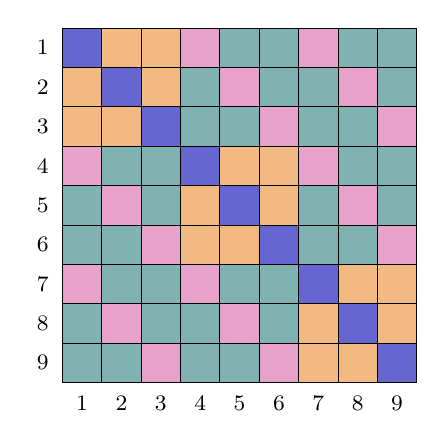
\begin{tikzpicture}[scale=0.5]
    \def\nm{9}
    \def\n{3} % Number of rows
    \def\m{3} % Number of columns
    % Draw the grid and fill colors
    \foreach \ik in {1,...,\n} {
        \foreach \jk in {1,...,\m} {
            \foreach \il in {1,...,\n} {
                \foreach \jl in {1,...,\m} {
                    % Compute the indexes
                    \pgfmathsetmacro{\k}{int(\ik + (\jk-1)*\n)}
                    \pgfmathsetmacro{\l}{int(\il + (\jl-1)*\n)}
                    % Color according to orbit type
                    \ifnum\ik=\il
                        \ifnum\jk=\jl
                            \fill[blue!70!black!60] (\l,-\k) rectangle ++(1,1);
                        \else
                            \fill[magenta!80!black!40] (\l,-\k) rectangle ++(1,1);
                        \fi
                    \else
                        \ifnum\jk=\jl
                            \fill[orange!90!black!50] (\l,-\k) rectangle ++(1,1);
                        \else
                            \fill[teal!80!black!50] (\l,-\k) rectangle ++(1,1); 
                        \fi
                    \fi
                    \draw[black, line width=0.3pt] (\l,-\k) rectangle ++(1,1);
                }
            }
        }
    }
    % Row and column labels
    \foreach \i in {1,...,\nm} {
        \node[left, font=\footnotesize] at (0.9,{-\i+0.5}) {\i};
        \node[below, font=\footnotesize] at (\i+0.5,-0.1 -\nm) {\i};
    }
\end{tikzpicture}
\end{center}


\subsection{~}

In the case of a linear invariant layer, for all $v\in\RF^{nm}$ and
$g\in G$ we have:
\begin{align*}
f(gv) & =f(v)\\
\Rightarrow w^Tgv+b & =w^Tv+b\\
\Rightarrow g^Tw & =w
\end{align*}
For $w\in\RF^{nm}$, this condition is equivalent to the condition on $b$ in the previous clause. 
Therefore, $w=c_2 \cdot \oneb$.

\subsection{~}

In the case of 3-tensors with the symmetric group is $S_{N_1}\times S_{N_2}\times S_{N_3}$
applied independently to each index axis of the tensor. We have: 
\begin{equation}
v=\vec(A) \,\,\,   v_k=a_{i_1,i_2,i_3}
,
\end{equation}
where $k=i_1+N_1(i_2-1)+N_1N_2(i_3-1)$. Define $k=i_1^{k}+N_1(i_2^{k}-1)+N_1N_2(i_3^{k}-1)$
and $l=i_1^{l}+N_1(i_2^{l}-1)+N_1N_2(i_3^{l}-1)$. We will
have the same derivation as in the previous clause \ref{subsec:q21},
thus 
\begin{align*}
W_{k,l} & =W_{g(k),g(l)}
\end{align*}
The indexes $\left(k,l\right)$ can transform to 
\begin{align*}
k' & =g_1(i_1^{k})+N_1(g_2(i_2^{k})-1)+N_1N_2(g_3(i_3^{k})-1)\\
l' & =g_1(i_1^{l})+N_1(g_2(i_2^{l})-1)+N_1N_2(g_3(i_3^{l})-1)
\end{align*}
where the equivalence relations follow the same pattern as before,
thus the orbits are 
\begin{equation}
\bigwedge_{n=1}^{3} i_n^{k}{}_{=}^{\neq}i_n^{l}
.    
\end{equation}
As a result, the orbits are:
\begin{align*}
O_{=i_1=i_2=i_3} & :i_1^{k}=i_1^{l},i_2^{k}=i_2^{l},i_3^{k}=i_3^{l}\\
O_{=i_1=i_2\neq i_3} & :i_1^{k}=i_1^{l},i_2^{k}=i_2^{l},i_3^{k}\neq i_3^{l}\\
O_{=i_1\neq i_2=i_3} & :i_1^{k}=i_1^{l},i_2^{k}\neq i_2^{l},i_3^{k}=i_3^{l}\\
\vdots &\\
O_{\neq i_1 \neq i_2\neq i_3} & :i_1^{k}\neq i_1^{l},i_2^{k}\neq i_2^{l},i_3^{k}\neq i_3^{l}
\end{align*}

For $N_1=N_2=N_3=3$, we obtain $W\in\RF^{27\times27}$ and $b\in\RF^{27}$.

\begin{center}
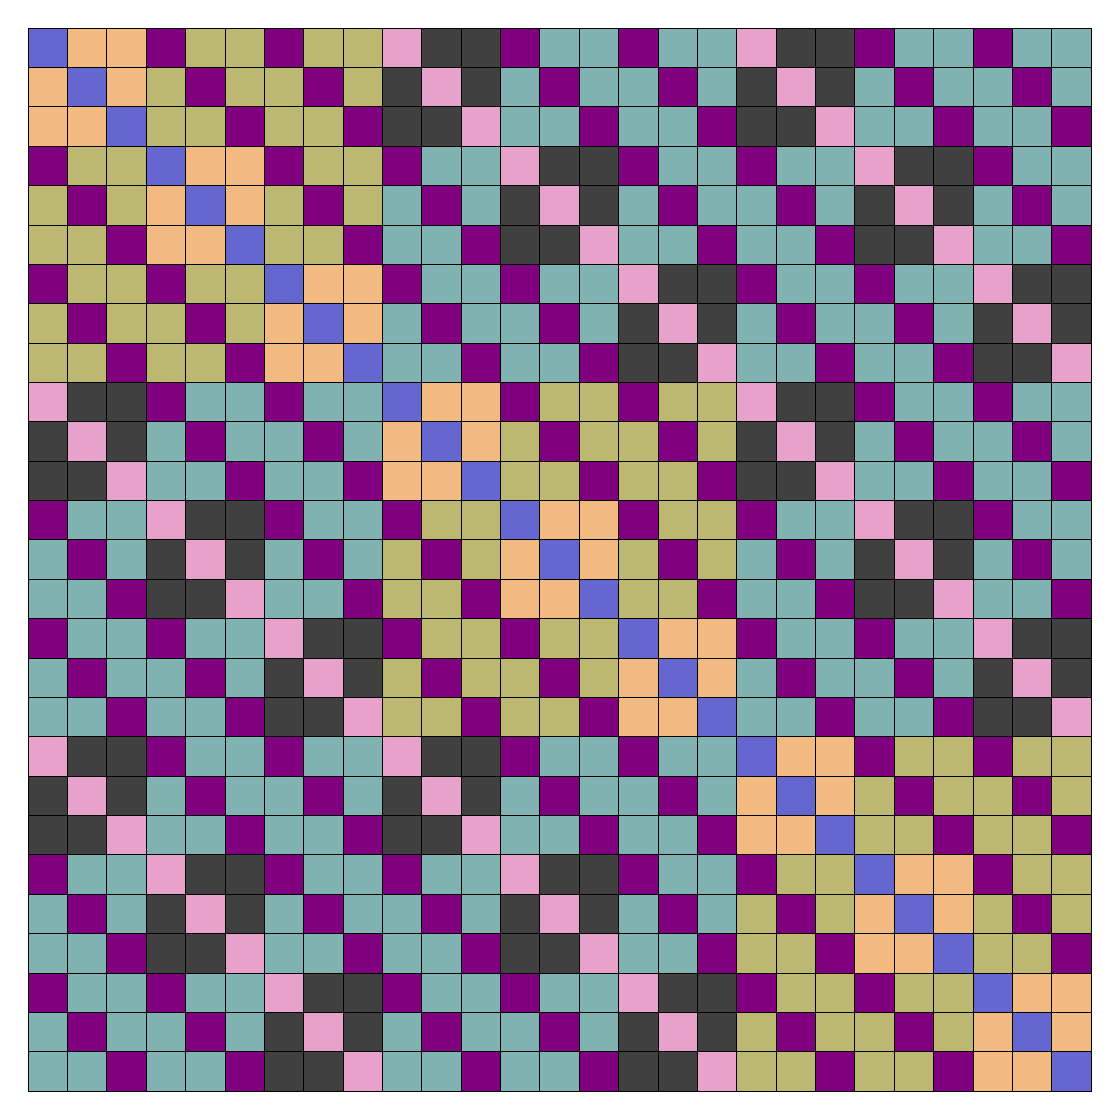
\begin{tikzpicture}[scale=0.5]
    \def\N{3} % Number of rows
    \def\M{3} % Number of columns
    \def\Q{3}
    \foreach \ik in {1,...,\N} {
        \foreach \jk in {1,...,\M} {
            \foreach \qk in {1,...,\Q} {
                \foreach \il in {1,...,\N} {
                    \foreach \jl in {1,...,\M} {
                        \foreach \ql in {1,...,\Q} {
                            % Compute the indexes
                            \pgfmathsetmacro{\k}{int(\ik + (\jk-1)*\N + (\qk-1)*\N*\M)}
                            \pgfmathsetmacro{\l}{int(\il + (\jl-1)*\N + (\ql-1)*\N*\M)}
                            % Color according to orbit type
                            \ifnum\ik=\il
                                \ifnum\jk=\jl
                                    \ifnum\qk=\ql
                                        \fill[blue!70!black!60] (\l,-\k) rectangle ++(1,1);
                                    \else
                                        \fill[magenta!80!black!40] (\l,-\k) rectangle ++(1,1);
                                    \fi
                                \else
                                    \ifnum\jk=\jl
                                        \ifnum\qk=\ql
                                            \fill[orange!90!black!50] (\l,-\k) rectangle ++(1,1);
                                        \else
                                            \fill[brown!80!black!50] (\l,-\k) rectangle ++(1,1);
                                        \fi
                                    \else
                                        \fill[red!50!blue] (\l,-\k) rectangle ++(1,1);
                                    \fi
                                \fi
                            \else
                                \ifnum\jk=\jl
                                    \ifnum\qk=\ql
                                        \fill[orange!90!black!50] (\l,-\k) rectangle ++(1,1);
                                    \else
                                        \fill[darkgray] (\l,-\k) rectangle ++(1,1);
                                    \fi
                                \else
                                    \ifnum\qk=\ql
                                        \fill[olive!80!black!50] (\l,-\k) rectangle ++(1,1);
                                    \else
                                        \fill[teal!80!black!50] (\l,-\k) rectangle ++(1,1);
                                    \fi
                                \fi
                            \fi
                            % Draw the rectangle border
                            \draw[black, line width=0.3pt] (\l,-\k) rectangle ++(1,1);
                        }
                    }
                }
            }
        }
    }
\end{tikzpicture}
\end{center}
    

\section{~ }

\section{~}
\end{document}
